\documentclass[10pt,a4paper]{article}
\usepackage[utf8]{inputenc}

% Define the page margin
\usepackage[margin=3cm]{geometry}

% Better typography (font rendering)
\usepackage{microtype}

% Math environments and macros
\usepackage{amsmath}
\usepackage{amsfonts}
\usepackage{amssymb}
\usepackage{amsthm}

% Define \includegraphics to include graphics
\usepackage{graphicx}

% Draw graphics from a text description
\usepackage{tikz}

% Syntax highlighting
\usepackage{minted}

% Set global minted options
\setminted{linenos, autogobble, frame=lines, framesep=2mm}

% Import the comment environment for orgtbl-mode
\usepackage{comment}

% Do not indent paragraphs
\usepackage{parskip}

\title{Databases, Sheet 12}
\author{Marten Lienen (03670270)}

\begin{document}

\maketitle

\section*{Exercise 1}

\begin{figure}[h]
  \centering
  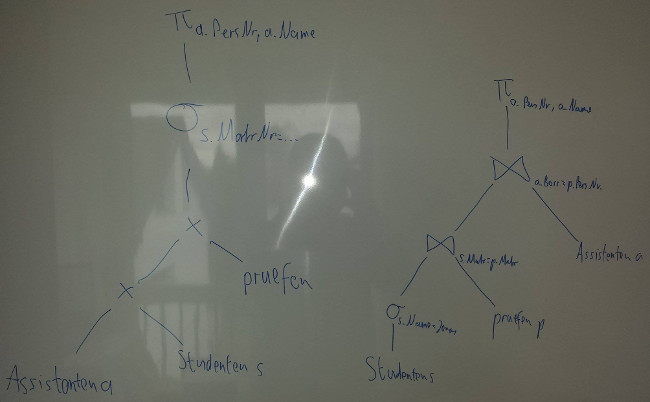
\includegraphics[width=\textwidth]{sheet-12/exercise-1}
  \caption{Exercise 1}
\end{figure}

\section*{Exercise 2}

\subsection*{Part 1)}

\begin{minted}{sql}
  SELECT *
  FROM Flughaefen f1, Flughaefen f2, Flughaefen f3, Verbindungen v1, Verbindungen v2
  WHERE
    f1.Stadt = "New-York" AND f2.Stadt NOT IN ("New-York", "Sydney") AND f3.Stadt = "Sydney" AND
    v1.von = f1.Code AND v1.nach = f2.Code AND v2.von = f2.Code AND v2.nach = f3.Code
\end{minted}

\subsection*{Part 2)}

\begin{figure}[h]
  \centering
  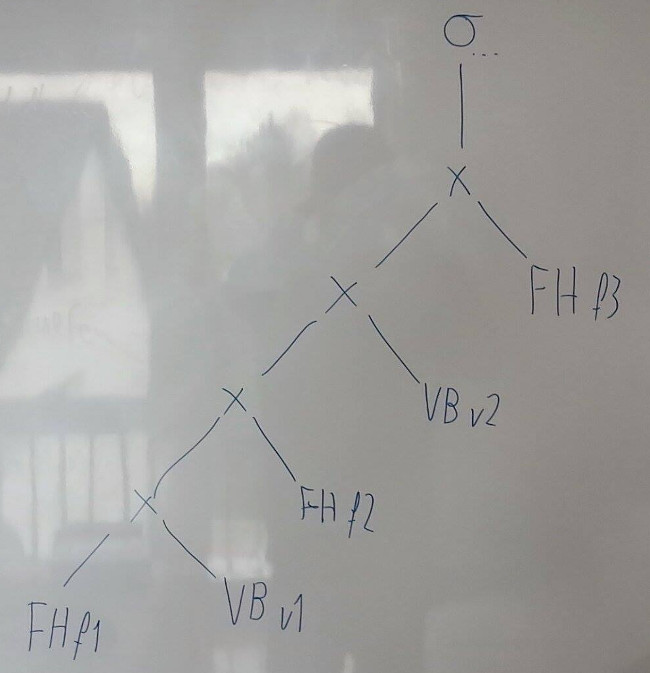
\includegraphics[width=\textwidth]{sheet-12/exercise-2-2}
  \caption{Exercise 2.2}
\end{figure}

\subsection*{Part 3)}

\begin{figure}[h]
  \centering
  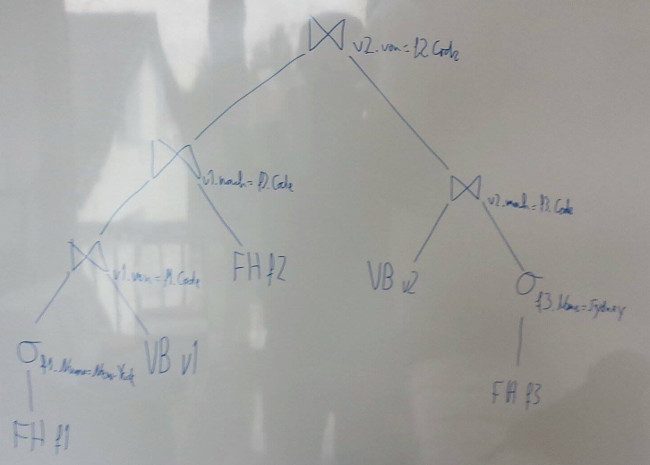
\includegraphics[width=\textwidth]{sheet-12/exercise-2-3}
  \caption{Exercise 2.3}
\end{figure}

\section*{Exercise 3}

\subsection*{Part a)}

Ein Equi-Join ist ein Join mit einer oder mehreren Gleichheitsbedingungen.

\subsection*{Part b)}

Nur bei Gleichheit, weil nur aus Gleichheit folgt, dass Tupel auch denselben Hash-Wert bekommen.

\subsection*{Part c)}

Bucket-Sort mit den Personennummern der Professoren, weil es von diesen wahrscheinlich weniger gibt als Räume.

\subsection*{Part d)}

Unmöglich, weil er ansonsten beliebig große Tabellen in konstanter Zeit materialisieren könnte ($A = \{ 1 \}$, $B = \{ 1, \dots, n \}$).

\section*{Exercise 4}

\begin{figure}[h]
  \centering
  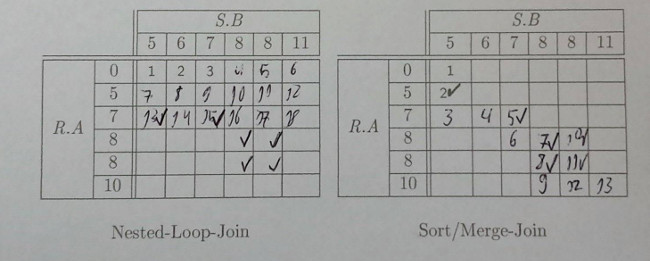
\includegraphics[width=\textwidth]{sheet-12/exercise-4}
  \caption{Exercise 4}
\end{figure}

\end{document}
